\documentclass[11pt]{article}
\usepackage[utf8]{inputenc}	% Para caracteres en español
\usepackage{amsmath,amsthm,amsfonts,amssymb,amscd}
\usepackage{multirow,booktabs}
\usepackage[table]{xcolor}
\usepackage{fullpage}
\usepackage{lastpage}
\usepackage{enumitem}
\usepackage{fancyhdr}
\usepackage{mathrsfs}
\usepackage{wrapfig}
\usepackage{setspace}
\usepackage{hyperref}
\usepackage{calc}
\usepackage{multicol}
\usepackage{cancel}
\usepackage[retainorgcmds]{IEEEtrantools}
\usepackage[margin=3cm]{geometry}
\usepackage{amsmath}
\newlength{\tabcont}
\setlength{\parindent}{0.0in}
\setlength{\parskip}{0.05in}
\usepackage{empheq}
\usepackage{framed}
\usepackage[most]{tcolorbox}
\usepackage{xcolor}
\colorlet{shadecolor}{orange!15}
\parindent 0in
\parskip 12pt
\geometry{margin=1in, headsep=0.25in}
\theoremstyle{definition}
\usepackage{pdfpages}
\newtheorem{defn}{Definition}
\newtheorem{reg}{Rule}
\newtheorem{exer}{Exercise}
\newtheorem{note}{Note}
\usepackage{fancyhdr}\usepackage{xcolor}\usepackage{amsmath}\usepackage{amssymb}\pagestyle{fancy}\rhead{}
\newtheorem{theorem}{Theorem}[subsection]
\theoremstyle{definition}
\newtheorem{definition}[theorem]{Definiton}
\newtheorem{example}[theorem]{Example}
\newtheorem{corollary}[theorem]{Corollary}
\newtheorem{lemma}[theorem]{Lemma}
\title{Chapter 9 Review Notes}
\begin{document}
\thispagestyle{empty}
{\LARGE \bf MSE 160 Lecture Notes}\\
{\large Hei Shing Cheung}\\
Molecules and Materials, Winter 2024 \hfill MSE 160\\
\begin{center}
\textit{"In this class we are mostly understanding solids''} \\ - Prof. \textsc{Scott Ramsay}
\end{center}
\vspace{10pt}
\section{Mechanical Behavior}
\paragraph{Classes of Materials} In this class, we look at three classes of materials (non-exhaustive):
\begin{itemize}
    \item \textbf{Metal} held together with metallic bonds, typically \textbf{ductile} and \textbf{conductive}.
    \item \textbf{Ceramics}  (often metal oxides [excp: diamond]) held together via covalent \& ionic bonds, typically \textbf{brittle} and \textbf{insulating}.
    \item \textbf{Polymers} Molecules (often hydrocarbons) typically \textbf{ductile} and \textbf{insulating}
\end{itemize}
\paragraph{Engineering Stress} For normal stress, we know that:
\begin{equation}
    \sigma = \frac{F}{A_0}
\end{equation}
\paragraph{Engineering Strein} Also:
\begin{equation}
    \epsilon = \frac{\Delta l}{l_0}
\end{equation}
\paragraph{Young's Moduclus} For elastic deformation, $E$, is given, by Hooke's Law, as follows:
\begin{equation}
    \sigma = E \epsilon
\end{equation}
\paragraph{Tensile Test} We apply force as to the ends of a dogbone-sample, with $l_0$ being the gauge length and $A_0$ being the area of the cross-section at the middle. 
\paragraph{Tensile Strein} Maximum tensile strain on the engineeging stress-strain curve.
\subsection{Understanding Elastic Properties in terms of Atomic Configuration}
\paragraph{Atomic Configuration} We can understand the elastic properties of a material by looking at the atomic configuration. Skemetically, we can represent the atomic configuration as a spring system:
\begin{enumerate}
    \item \textbf{Intial - Before Loading} Atoms are in equilibrium, with the interatomic forces being balanced.
    \item \textbf{Loading} We apply a force to the material, causing the atoms to move from their equilibrium positions. The bond stretches and the atoms move further apart.
    \item \textbf{Unloading} We remove the force, causing the atoms to return to their equilibrium positions. 
\end{enumerate}
\paragraph{Atom Positions} Elastic modulus is dependent on the atomic interatomic bonding force. Thus, The elastic modulus is prootionaly to the slope of the interatomic force-seperation curve.
\paragraph{Force-Seperation Curve} The force-seperation curve is a plot of the force between two atoms as a function of the distance between them. The slope of the curve is proportional to the elastic modulus near the equilibrium position.

\begin{figure}[h]
    \centering
    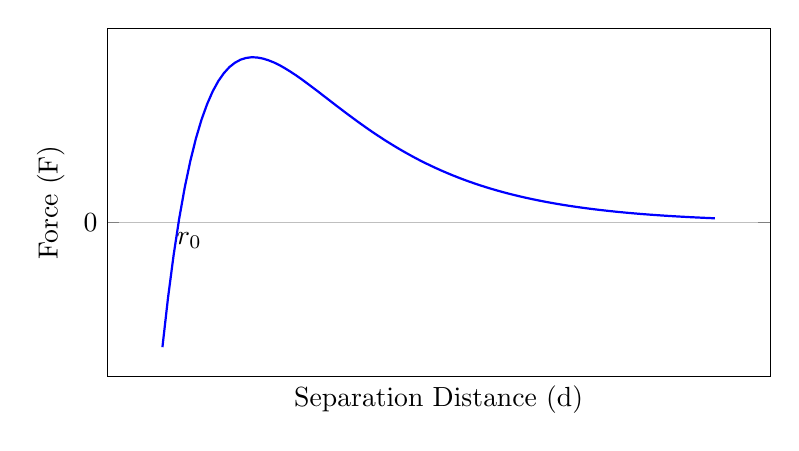
\begin{tikzpicture}
        \begin{axis}[
            xlabel={Separation Distance (d)},
            ylabel={Force (F)},
            grid=major,
            width=10cm,
            height=6cm,
            domain=-0.3:10,
            samples=100,
            xtick = \empty,
            ytick = {0}
        ]
        \addplot[blue, thick] {exp(-x/2) - exp(-x)};
        \node at (axis cs:0.2,0) [anchor=north] {$r_0$};
        
    \end{axis}
    \end{tikzpicture}
    \caption{Force-Separation Curve (Lennard-Jones Force)}
    \label{fig:force-separation}
\end{figure}
\begin{equation}
    E \propto \frac{dF}{dr} \Bigg|_{r_0}
\end{equation}
\begin{definition}[Equilibrium interatomic seperation distance]
The equilibrium interatomic seperation distance, $r_0$, is the distance between two atoms at which the interatomic force is zero. This is due to the interatomic forces being the sum of attractive and repulsive forces.
\end{definition}
\paragraph{Elastic Modulus} Thus, strongly bonded materials have a higher elastic modulus and the slope of the force-seperation curve is steeper at $r_0$.
\subsection{Understanding Other Properties in terms of Atomic Configuration}
\paragraph{Potential Energy-Separation Curve} The potential energy-seperation curve is a plot of the potential energy between two atoms as a function of the distance between them. The potential energy is the area under the force-seperation curve.
\paragraph{Depth of the Minimum Energy Well} The depth of the minimum energy well, $E_0$, is the energy required to break the bond between two atoms. This is the energy required to move the atoms from the equilibrium position to infinity. It is proportional to the melting temperature of the material.
\begin{figure}[h]
    \centering
    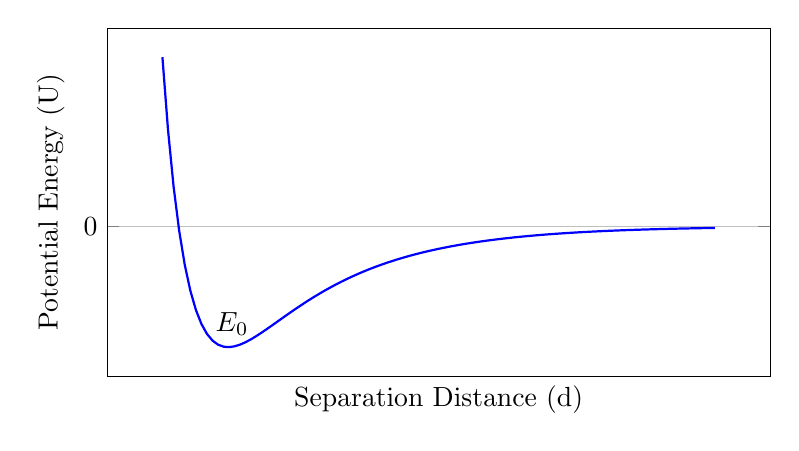
\begin{tikzpicture}
        \begin{axis}[
            xlabel={Separation Distance (d)},
            ylabel={Potential Energy (U)},
            grid=major,
            width=10cm,
            height=6cm,
            domain=-0.3:10,
            samples=100,
            xtick = \empty,
            ytick = {0}
        ]
        \addplot[blue, thick] {-exp(-x/2) + exp(-x)^2};
        \node at (axis cs:1,-0.3) [anchor=north] {$E_0$};
        
    \end{axis}
    \end{tikzpicture}
    \caption{Potential Energy-Separation Curve}
    \label{fig:potential-energy}
\end{figure}
\paragraph{Coefficient of Thermal Expansion} The coefficient of thermal expansion, $\alpha$, is the fractional change in length per degree change in temperature. 
\paragraph{Depth of Potential Energy Curve} The deeper the potential energy curve, the higher the melting temperature and more symetric the curve near $E_0$. This would give the follwoing three properties:
\begin{enumerate}
    \item \textbf{Higher Melting Temperature} The higher the melting temperature, the deeper the potential energy curve.
    \item \textbf{Higher Elastic Modulus} The steeper the slope of the force-seperation curve at $r_0$, the higher the elastic modulus.
    \item \textbf{Lower Coefficient of Thermal Expansion} The more symetric the potential energy curve near $E_0$, the lower the coefficient of thermal expansion.
\end{enumerate}
\subsection{Shear and Tensile Stress}
\subsubsection{Shear}
\paragraph{Shear Stress} Shear stress is the force per unit area acting parallel to the surface. It is given by:
\begin{equation}
    \tau = \frac{F}{A_0}
\end{equation}
\paragraph{Shear Strain} Shear strain is the change in angle between two lines originally perpendicular to each other. It is given by:
\begin{equation}
    \gamma = \frac{\Delta l}{l_0} \approx \tan \theta \approx \theta = \frac{\pi}{2} - \phi
\end{equation}
\paragraph{Shear Modulus} The shear modulus, $G$, is the ratio of shear stress to shear strain. It is given by:
\begin{equation}
    \tau = G \gamma
\end{equation}
\paragraph{Relationship between Shear and Tensile Modulus} The shear modulus is related to the tensile modulus by the following equation:
\begin{equation}
    G = \frac{E}{2(1+\nu)}
\end{equation}
where $\nu$ is the Poisson's ratio.
\paragraph{Poisson's Ratio} Poisson's ratio, $\nu$, is the ratio of lateral strain to axial strain. It is given by:
\begin{equation}
    \nu = -\frac{\epsilon_{\text{lat}}}{\epsilon_{\text{axial}}}
\end{equation}
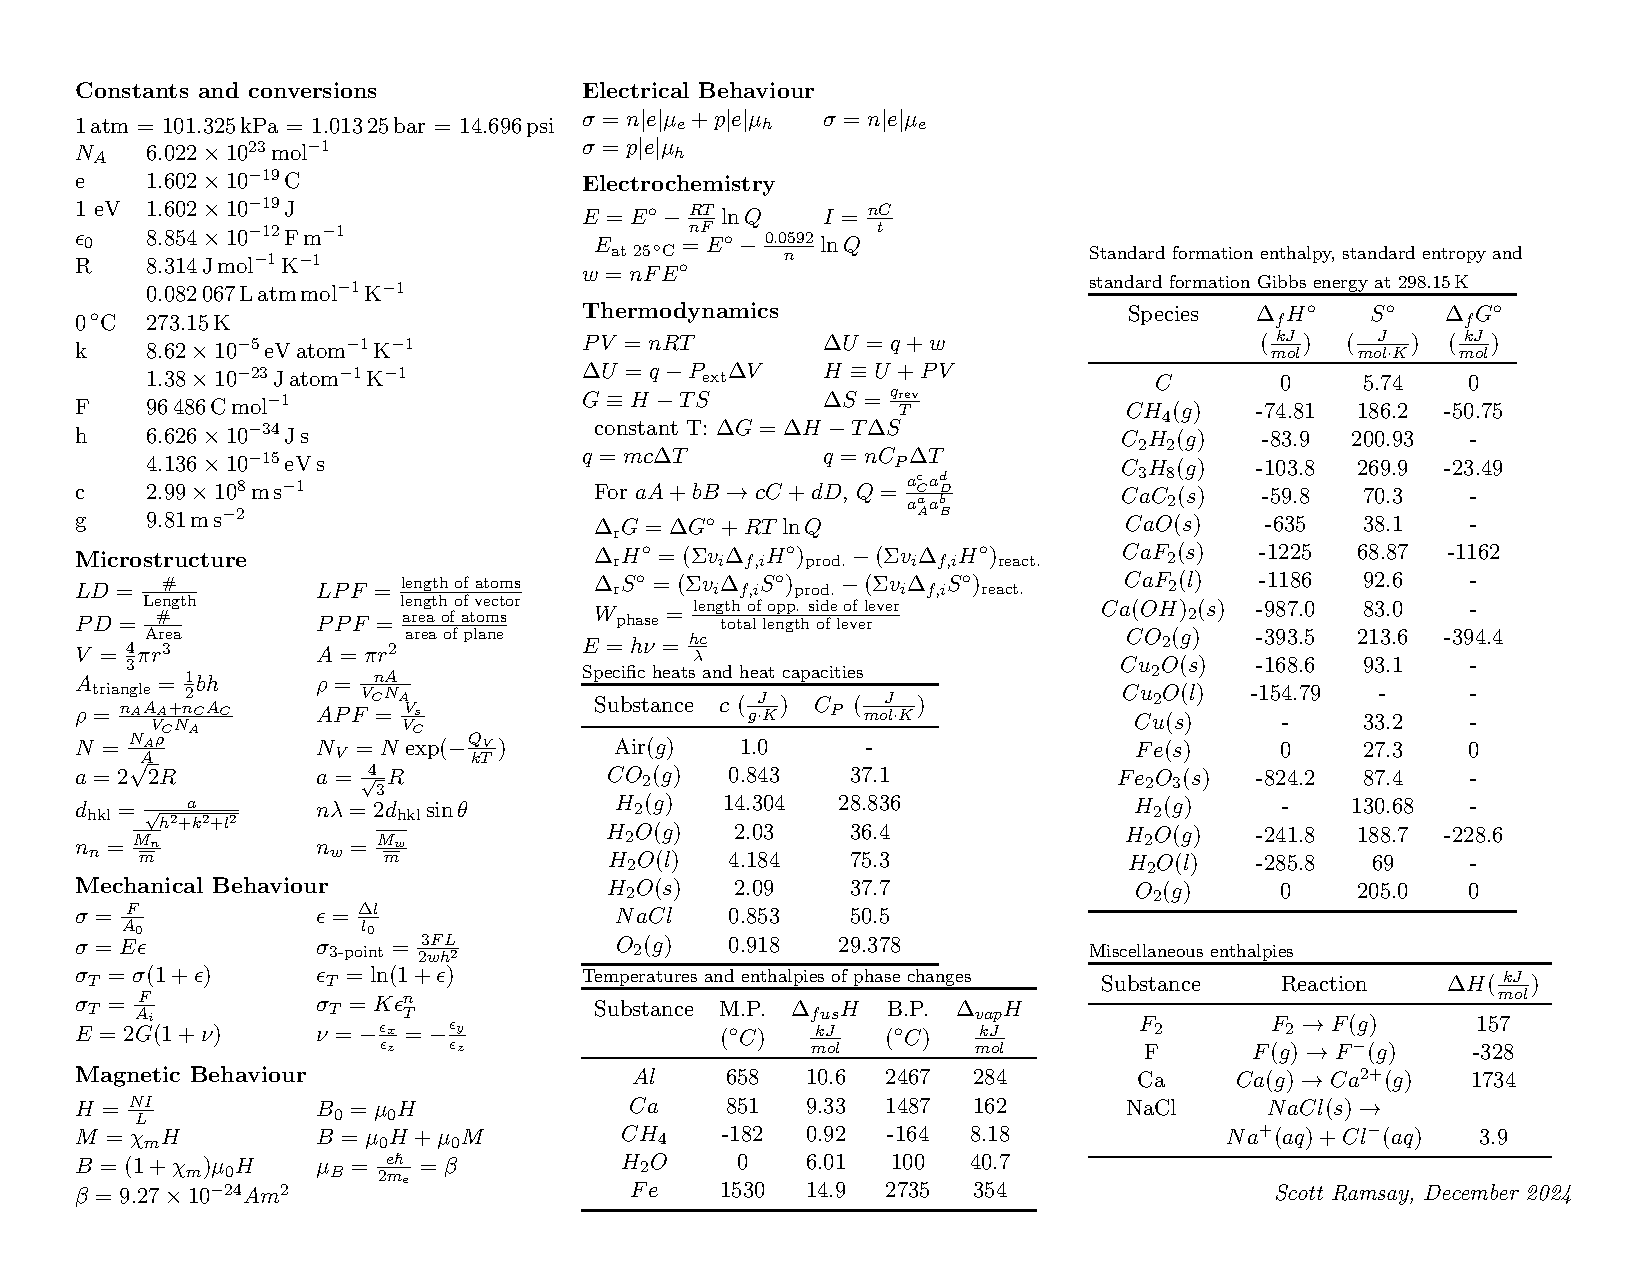
\includepdf[pages=-, angle=90]{EquationSheet.pdf}
\end{document}